
%
%	Section 1
%

\section{Introduction}\label{Section_Introd}
\Headerfooter{Introduction}

\subsection{Neutrino}
\vs\hs Neutrinos, which are Fermions with spin of 1$/$2, are classified as leptons that do not participate in the strong interaction in the Standard Model (SM) of the particle physics.
Moreover, neutrinos do not have charge, and the neutrino mass is so tiny that the gravitational interaction can be ignored.
Therefore, neutrinos interact with other particles only via the weak interaction, and are difficult to observe.
The name "neutrino" was named by E. Fermi in 1933~\cite{HistoryOfNeutrino}.
The name comes from the "neutral" that means the zero charge, and "ino" that means small in Italian.
Currently, we know that there are three flavors of neutrinos: electron neutrino, muon neutrino, and tau neutrino.\\
\hs The existence of neutrinos was suggested by W. Pauli in 1930~\cite{HistoryOfNeutrino}.
Once, the energy spectrum of the electron emitted by the beta decay was expected to be the line spectrum.
However, in 1914, J. Chadwick found that the energy spectrum was not the line spectrum but the continuous spectrum~\cite{1914Chadwick}.
To explain the continuous spectrum of the electron reported by Chadwick, Pauli claimed that an unknown particle with spin of 1$/$2 and zero charge is emitted in the beta decay in addition to the electron.
In 1956, more than 20 years after Pauli proposed the existence of neutrinos, (electron anti)neutrinos produced in nuclear reactors were discovered by F. Reines and C. Cowan~\cite{1956Reines}.
In 1962, muon neutrinos were discovered in the accelerator experiment by L. Lederman, M. Schwartz, and J. Steinberger~\cite{1962Danby}.
In 2001, tau neutrinos were discovered in the DONUT (Direct Observation of NU Tau) experiment~\cite{2001Kodama}.

\subsection{Neutrino oscillation}
\vs\hs In the SM, the neutrino mass is zero~\cite{2022Workman}.
However, in 1998, the evidence for the neutrino oscillation was discovered in the Super-Kamiokande and it was proved that the neutrino mass is not zero~\cite{1998Fukuda}.
Neutrino oscillation is a phenomenon that the flavor of neutrino changes while the neutrino passes through a space.\\
\hs Here the neutrino oscillation in vacuum is considered.
The flavor eigenstate $\ket{\nu_{\alpha}}$ is represented by the superposition of the mass eigenstate $\ket{\nu_{i}}$,
\begin{eqnarray}
	\ket{\nu_{\alpha}}=\sum_{i=1}^{n} U_{\alpha i}^{*}\ket{\nu_{i}},
\end{eqnarray}
where $n$ ($=3$) is the number of neutrino species and $U$ is a 3$\,\times\,$3 unitary matrix, called the Pontecorvo-Maki-Nakagawa-Sakata (PMNS) mixing matrix.
This matrix consists of four independent parameters (three mixing angles, $\theta_{12}$, $\theta_{23}$, and $\theta_{13}$, and one phase angle $\delta_{{\rm CP}}$),
\begin{eqnarray}
	U&=&\left(
	\begin{array}{ccc}
		1&0&0\\
		0&c_{23}&s_{23}\\
		0&-s_{23}&c_{23}
	\end{array}
	\right)
	\left(
	\begin{array}{ccc}
		c_{13}&0&s_{13}e^{-i\delta_{{\rm CP}}}\\
		0&1&0\\
		-s_{13}e^{i\delta_{{\rm CP}}}&0&c_{13}
	\end{array}
	\right)
	\left(
	\begin{array}{ccc}
		c_{12}&s_{12}&0\\
		-s_{12}&c_{12}&0\\
		0&0&1
	\end{array}
	\right) \nonumber \\
	&=&\left(
	\begin{array}{ccc}
		c_{12}c_{13}&s_{12}c_{13}&s_{13}e^{-i\delta_{{\rm CP}}}\\
		-s_{12}c_{23}-c_{12}s_{23}s_{13}e^{i\delta_{{\rm CP}}}&c_{12}c_{23}-s_{12}s_{23}s_{13}e^{i\delta_{{\rm CP}}}&s_{23}c_{13}\\
		s_{12}s_{23}-c_{12}c_{23}s_{13}e^{i\delta_{{\rm CP}}}&-c_{12}s_{23}-s_{12}c_{23}s_{13}e^{i\delta_{{\rm CP}}}&c_{23}c_{13}
	\end{array}
	\right),
\end{eqnarray}
where $c_{ij}\equiv\cos\theta_{ij}$ and $s_{ij}\equiv\sin\theta_{ij}$.
After traveling a distance $L$ ($\simeq ct$ for relativistic neutrinos), the flavor eigenstate evolves as
\begin{eqnarray}
	\ket{\nu_{\alpha}(t)}=\sum_{i=1}^{n} U_{\alpha i}^{*}\ket{\nu_{i}(t)},
\end{eqnarray}
where $\ket{\nu_{i}(t)}=e^{-iE_{i}t}\ket{\nu_{i}(0)}$ ($E_{i}$ is the energy of the neutrino mass eigenstate $\nu_{i}$).
At that time, the probability of being observed as the flavor eigenstate $\ket{\nu_{\beta}}$ is
\begin{eqnarray}\label{Introd_Eq_Prob}
	P_{\alpha\beta}=|\braket{\nu_{\beta}|\nu_{\alpha}(t)}|^{2}=\Bigg|\sum_{i=1}^{n}\sum_{j=1}^{n} U_{\alpha i}^{*}U_{\beta j}\braket{\nu_{j}|\nu_{i}(t)}\Bigg|^{2}.
\end{eqnarray}
Here, neutrinos are relativistic, thus $p_{i} \simeq p_{j} \equiv p \simeq E$. Therefore, $E_{i}$ can be approximated as
\begin{eqnarray}\label{Introd_Eq_E}
	E_{i} = \sqrt{p_{i}^{2}+m_{i}^{2}} = p_{i}\sqrt{1+{m_{i}^{2} \over p_{i}^{2}}} \simeq p_{i}\Bigg(1+{m_{i}^{2} \over 2p_{i}^{2}}\Bigg) \simeq E+{m_{i}^{2} \over 2E}.
\end{eqnarray}
Using Equation (\ref{Introd_Eq_E}) and the orthogonality of the mass eigenstates, $\braket{\nu_{j}|\nu_{i}}=\delta_{ij}$, Equation (\ref{Introd_Eq_Prob}) can be expressed as
\begin{eqnarray}
	P_{\alpha\beta}=\delta_{\alpha\beta}-4\sum_{i<j}^{n} {\rm Re}[U_{\alpha i}U_{\beta i}^{*}U_{\alpha j}^{*}U_{\beta j}]\sin^{2}X_{ij}+2\sum_{i<j}^{n} {\rm Im}[U_{\alpha i}U_{\beta i}^{*}U_{\alpha j}^{*}U_{\beta j}]\sin 2X_{ij},
\end{eqnarray}
where
\begin{eqnarray}
	X_{ij} = {(m_{i}^{2}-m_{j}^{2})L \over 4E} \equiv {\Delta m_{ij}^{2}L \over 4E} = 1.267{\Delta m_{ij}^{2} \over {\rm eV}^{2}}{L/E \over {\rm m}/{\rm MeV}}.
\end{eqnarray}
The neutrino oscillation between two neutrino species in vacuum is described in Appendix~\ref{AppA}.
Moreover, the neutrino oscillation in matter is described in Ref.~\cite{1989Kuo}.\\
\hs From the above calculation, it can be seen that the neutrino oscillation can be described by six parameters ($\theta_{12}$, $\theta_{23}$, $\theta_{13}$, $\Delta m_{21}^{2}$, $\Delta m_{32}^{2}$, and $\delta_{{\rm CP}}$).
These parameters can be measured by observing the oscillation phenomena of solar neutrinos, atmospheric neutrinos, reactor neutrinos, and accelerator neutrinos.
Table~\ref{Introd_Tab:Neu} shows the three-neutrino mixing parameters and $\delta_{{\rm CP}}$.
Currently, the values of $m_{1}$, $m_{2}$, and $m_{3}$ and the magnitude relationship between $m_{2}$ and $m_{3}$ are not yet known.
There are two possibilities of the neutrino mass ordering: Normal Ordering (NO, $m_{1}<m_{2}<m_{3}$) or Inverted Ordering (IO, $m_{3}<m_{1}<m_{2}$).

\begin{table}[h]
	\caption[Three-neutrino mixing parameters and $\delta_{{\rm CP}}$]{\label{Introd_Tab:Neu} Three-neutrino mixing parameters and $\delta_{{\rm CP}}$~\cite{PDG}. Here, $\theta_{ij}\in[0,\pi/2]$ and $\delta_{{\rm CP}}\in[0,2\pi]$.}
	\centering
	\vs
	\begin{tabular}{ll}
		\hline\hline
		$\sin^{2}\theta_{12}$&$0.307 \pm 0.013$\\
		$\sin^{2}\theta_{23}$ (NO)&$0.547\,^{+0.018}_{-0.024}$\\
		$\sin^{2}\theta_{23}$ (IO)&$0.534\,^{+0.021}_{-0.024}$\\
		$\sin^{2}\theta_{13}$&$(2.20 \pm 0.07) \times 10^{-2}$\\
		$\Delta m_{21}^{2}$&$(7.53 \pm 0.18) \times 10^{-5}\,{\rm eV}^{2}$\\
		$\Delta m_{32}^{2}$ (NO)&$(2.437 \pm 0.033) \times 10^{-3}\,{\rm eV}^{2}$\\
		$\Delta m_{32}^{2}$ (IO)&$(-2.519 \pm 0.033) \times 10^{-3}\,{\rm eV}^{2}$\\
		$\delta_{{\rm CP}}$&$1.23 \pm 0.21\,\pi\,{\rm rad}$\\
		\hline\hline
	\end{tabular}
\end{table}

\subsection{Supernova explosion}

\subsection{Current status of DSNB search}

\subsection{Neutrino-oxygen NCQE reactions}

\begin{figure}[tbp]
	\centering
	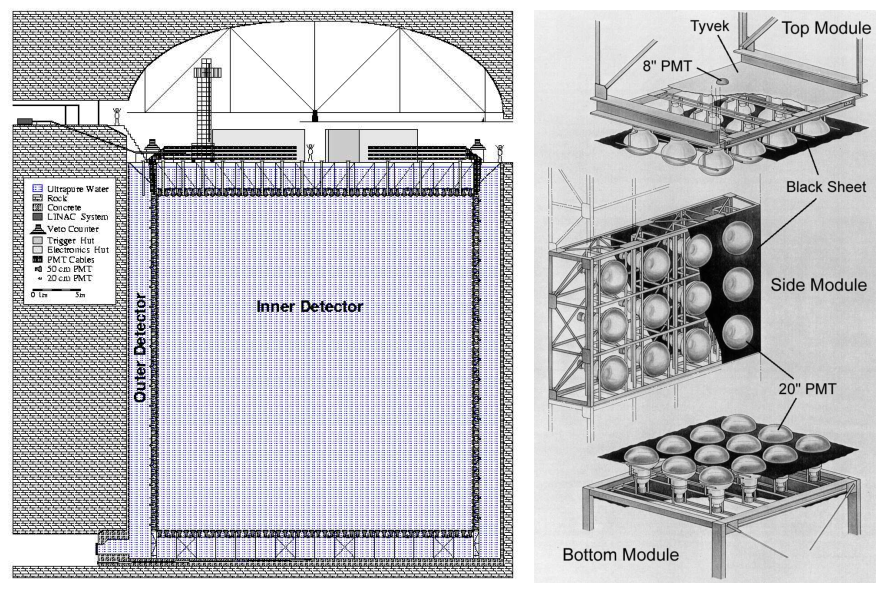
\includegraphics[width=14cm]{Figures/SK/SK_SM}
	\caption[Cross section of the SK detector and overview of supermodule frames]{\label{SK_SK_SM} Cross section of the SK detector (left) and overview of supermodule frames (right)~\cite{2003Fukuda}.}
\end{figure}

\newpage
